\begin{figure*}[t!]
  \centering
  \hspace{-8mm}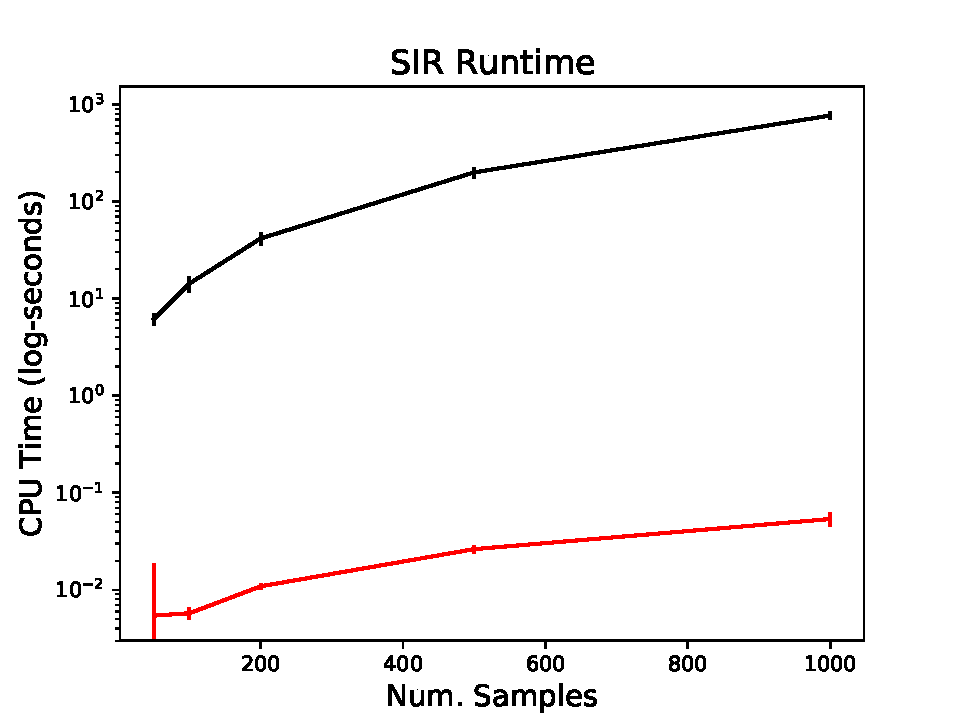
\includegraphics[width=0.28\textwidth]{sir_runtime_benchmark}
  \hspace{-4mm}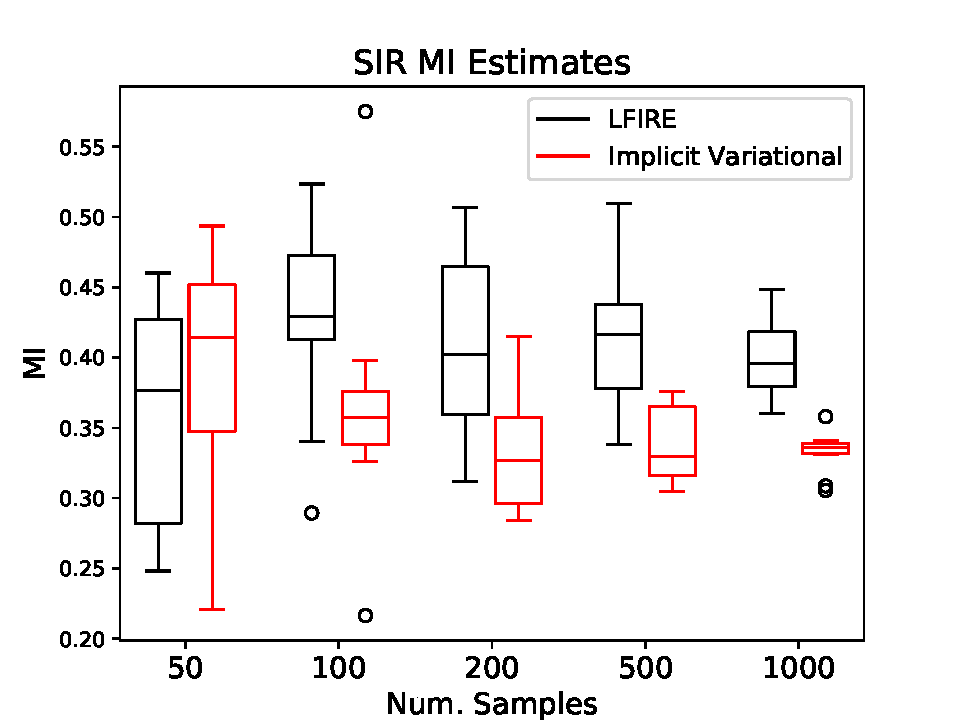
\includegraphics[width=0.28\textwidth]{sir_utility_benchmark}
  \hspace{-4mm}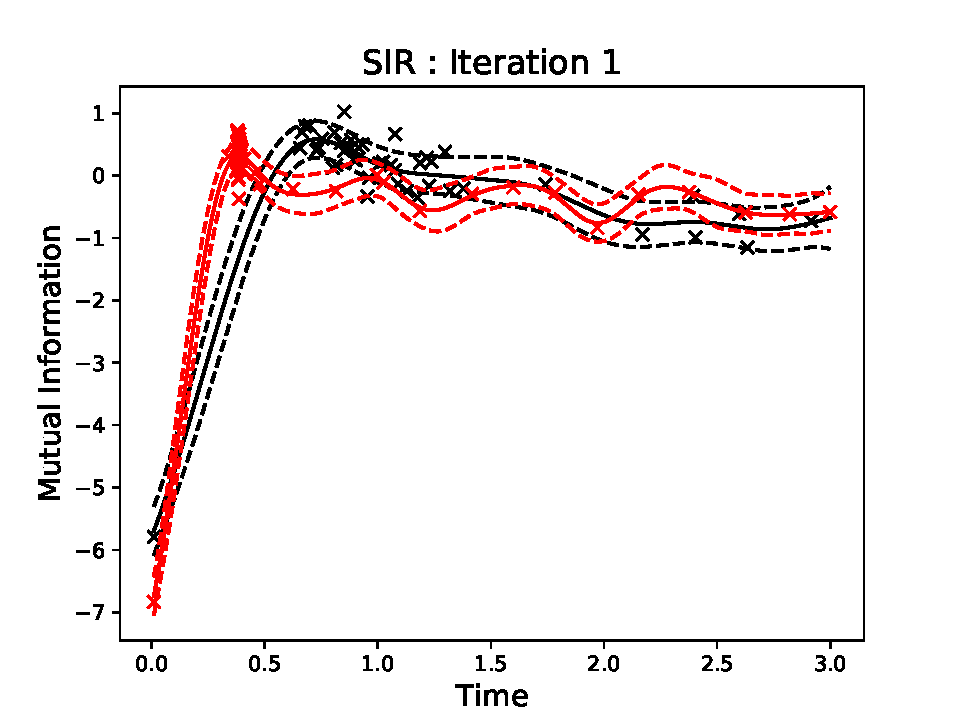
\includegraphics[width=0.28\textwidth]{sir_500p_K3_iter1}
  \hspace{-4mm}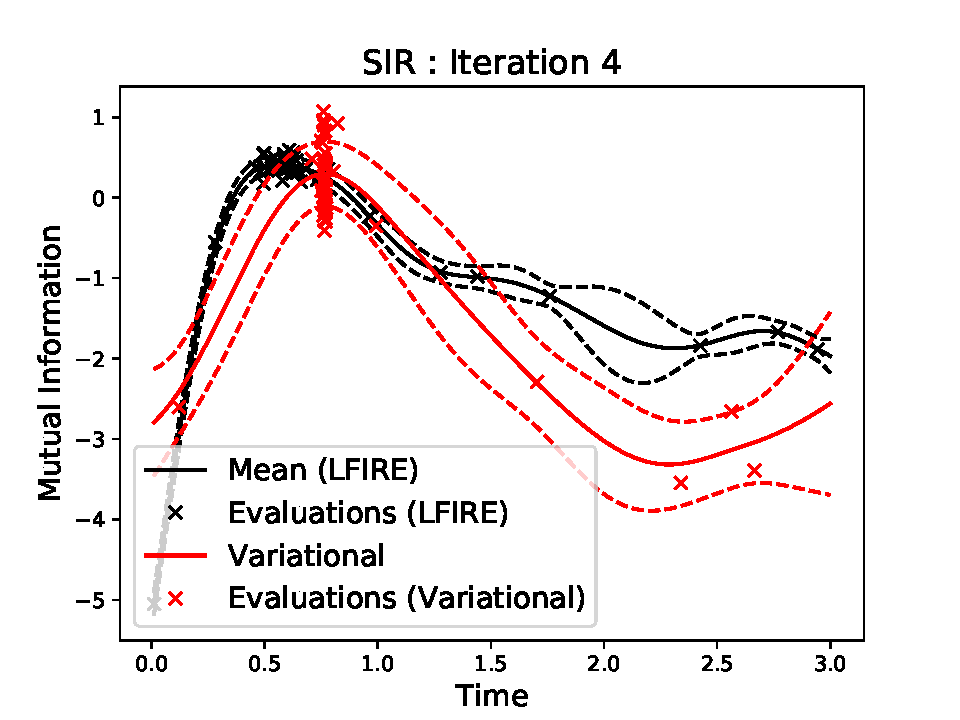
\includegraphics[width=0.28\textwidth]{sir_500p_K3_iter4}
  \caption{\small \textbf{SIR Sequetial Design.} Left plots show benchmark
    time and utility evaluation between LFIRE and the Variational
    estimator for a fixed design ($d=1.0s$) over 10 runs each at a
    range of sample sizes.  The variational estimator is orders of
    magnitude more efficient (\emph{left}) and shows lower variance at
    each sample (\emph{center-left}).  The first (\emph{center-right})
    and fourth (\emph{right}) sequential BED iterations yield
    comparable designs between both methods (GP posterior MI shown).}
  \label{fig:sir_results}
\end{figure*}

\paragraph{The SIR model} 
describes the time-evolution of infection in a fixed
population~\cite{kermack1927contribution, allen2008introduction}.  At
each time $t$ the population is divided into three components:
\emph{susceptible} $S(t)$, \emph{infected} $I(t)$, and
\emph{recovered} $R(t)$ according to the time-series,
\begin{align}
  S(t + \Delta_t) &= S(t) - \Delta I(t) \label{eq:s} \\
  I(t + \Delta_t) &= I(t) + \Delta I(t) - \Delta R(t) \\
  R(t + \Delta_t) &= R(t) + \Delta R(t) \label{eq:r}
\end{align}
\begin{wrapfigure}{r}{0.3\textwidth}
  \vspace*{-5mm}
  \centering
  \hspace*{-5mm}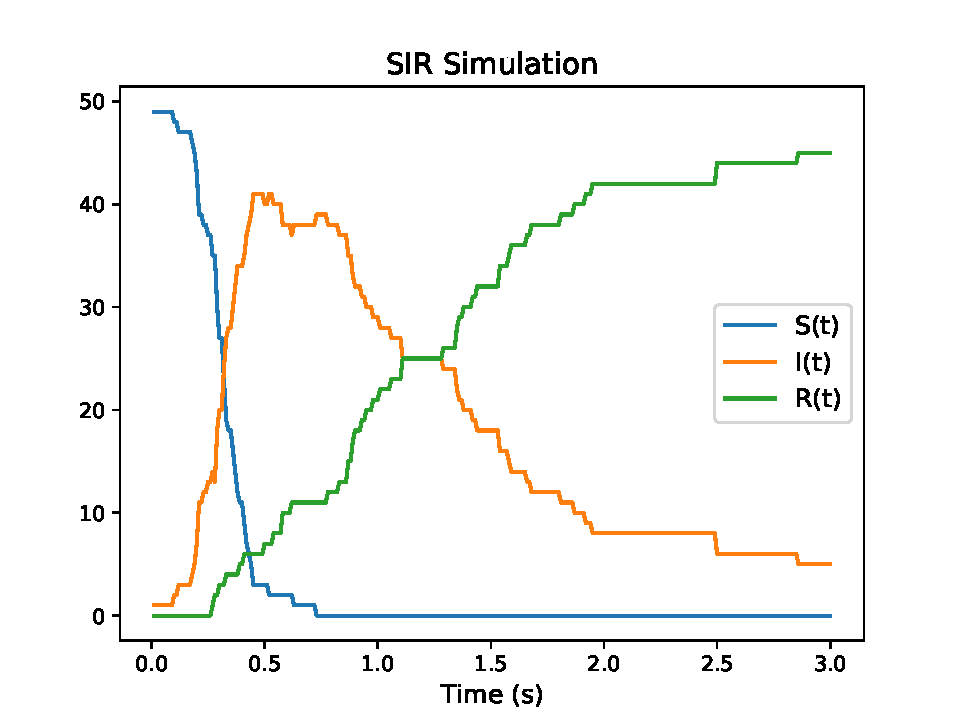
\includegraphics[width=0.35\textwidth]{sir_sim_beta_0p14_gamma_0p01}  
  \caption{\small SIR model simulation for $\beta = 0.14,
    \gamma=0.01$.}
  \vspace*{-5mm}
  \label{fig:sir_sim}
\end{wrapfigure}
At each time the change in infected $\Delta I(t)$ and recovered
$\Delta R(t)$ are Binomially distributed,
\[
  \Delta I(t) \sim \text{Binomial}\left(S(t), \frac{\beta
    I(t)}{N}\right), \quad
  \Delta R(t) \sim \text{Binomial}(I(t), \gamma)
\]
with unknown random parameters $\beta, \gamma \sim
\text{Uniform}(0,0.5)$.  Our simulations use a fixed discrete time
interval $\Delta_t = 0.01$ with a population $N=50$ and boundary
conditions $S(t=0) = N-1$, $I(t=0)=1$, and $R(t=0) =
0$. See \FIG\ref{fig:sir_sim} for an example of the SIR simulation.


\paragraph{Sequential Design} We select a time $t > 0$ with maximal
information about the parameters $\beta, \gamma$ as in, \mbox{$\argmax_t \, I\left(\{\beta, \gamma\} ; \{S(t),
I(t)\} \right)$}.
%% Early and late
%% stages are uninformative, since the population is largely uninfected
%% or recovered.  
We ignore $R$ in the MI quantity since it is deterministic via: $R(t)
= N - I(t) - S(t)$.  After choosing a time $t^*$ we observe $S(t^*) =
s$, $I(t^*) = \iota$, and $R(t^*) = r$.  In stage $K$ of sequential
(greedy) design we condition on $K-1$ previously-chosen times $t^*_1,
\ldots, t^*_{K-1}$ and their resulting observations $\{s_1^{K-1},
\iota_1^{K-1}\}$, denoted by the ``history'' set $\mathcal{H}_{K-1}$.  The
$K^{\text{th}}$ time is chosen to maximize,
\begin{equation}\label{eq:mi_sir}
  t_K^* = \argmax_{t > 0} \; I\left(\{\beta, \gamma\} ; \{S(t),
  I(t)\} \mid \mathcal{H}_K \right).
\end{equation}
Optimizing \EQN\eqref{eq:mi_sir} is complicated since the SIR lacks an
explicit likelihood \mbox{$p(S(t), I(t), R(t) \mid \beta, \gamma)$}--it is
defined implicitly through simulation of
\EQNS\eqref{eq:s}-\eqref{eq:r}.  Existing design approaches to
sequential design in this model~\cite{kleinegesse2021sequential} rely
on LFIRE~\cite{thomas2022likelihood} estimates of the ratio
$\frac{p(S, I, R \mid \beta, \gamma)}{p(S, I, R)}$ for calculating MI
in \EQN\eqref{eq:mi_sir}.

\paragraph{Fast and accurate variational estimates.} We compare our moment-matched
$\hat{I}_{m+\ell}$ MI estimator to the LFIRE estimator.  For
sequential design we use the implementation of Kleinegesse et
al.~(\citeyear{kleinegesse2021sequential}) which estimates MI based on
importance weighted expectations of the LFIRE ratio estimator.
\FIG\ref{fig:sir_results} shows that our moment matching estimates
achieve several orders of magnitude speedup (left) with comparable
estimates and reduced variance (left-center).  We note that our
estimates are based on the same samples as those used in LFIRE.  In
sequential greedy design we observe comparable time-point selections
across iterations as compared to that of Kleinegesse et
al. (center-right and right).  Note that Kleinegesse et al. report
only 4 design stages since the code is prohibitively slow for further
designs.  Using our estimator it is possible to conduct many more
design iterations in a fraction of the time.




% Our simulations use a fixed discrete time interval of $\Delta_t =
% 0.01$ units.  
